

% ----------------------------------------------------------
% Introdução (exemplo de capítulo sem numeração, mas presente no Sumário)
% ----------------------------------------------------------

\chapter[Introdução]{Introdução \showfont}
%\addcontentsline{toc}{chapter}{Introdução}
% ----------------------------------------------------------
\begin{flushright}
	\textit{``The curious paradox is that when I accept myself just as I am, then I can change.''}\\
	Carl Rogers
\end{flushright}


%\showfont
\newpage


\section[Some encoding tests]{\showfont}
\subsection{\showfont}
\subsubsection{\showfont}
\subsubsubsection{\showfont}


\textsf{textsf: \showfont} 

\textrm{textrm: \showfont}

\textnormal{textnormal: \showfont}

\textbf{textbf: \showfont} 

\textit{textit: \showfont}

footnote\footnote{\showfont}

% \emph{emphasize: \showfont} 

``Modelo Canônico \showfont''

\begin{itemize}
	\item \textrm{Roman family - \showfont }
	\item \textsf{Sans serif family - \showfont}
	\item \texttt{Typewriter/teletype family - \showfont}
	\item \textit{italics text - \showfont}
	\item \textsl{slanted text- \showfont}
	\item \textsc{small caps text- \showfont}	
\end{itemize}




mathnormal -  default: $\mathnormal{abcXYZ}$

mathrm - roman: $\mathrm{abcXYZ}$

mathbf - bold roman: $\mathbf{abcXYZ}$

mathsf - sans serif: $\mathsf{abcXYZ}$

mathit - text italic: $\mathit{abcXYZ}$

mathtt -  typewriter: $\mathtt{abcXYZ}$

mathcal - calligraphic: $\mathcal{XYZ}$


%\pagevalues

\begin{figure}
	\caption{Page layout for this document -  \showfont} \label{fig:ptrs}
	%\drawpage
	\setlayoutscale{0.4}
	%	\currentpage
	\drawparameterstrue
	\drawpage
	%	\pagedesign
	%	\pagevalues
\end{figure}


\begin{figure}
	\caption{Page layout values for this document} \label{fig:ptrsval}
	
	\pagevalues
\end{figure}



\begin{figure}
	\currentfootnote
	\drawparameterstrue
	%	\setlayoutscale{0.4}
	\drawfootnote
	\footnotevalues
	\caption{The current footnote layout}\label{fig:ftry}
\end{figure}	
	

\begin{figure}
	\drawparagraph
	\paragraphvalues
	\caption{Paragraph parameters}\label{fig:fpara}
\end{figure}


\begin{figure}
	\setlayoutscale{0.6}
	\drawparameterstrue
	\drawtoc
	\tocvalues
	\caption{Table of Contents entry parameters}\label{fig:tocp}
\end{figure}





A Tabela~\ref{tab:a} mostra mais informações do template BU.

\begin{table}[!htb]
	\begin{center}
		\caption{Formatação do texto. \showfont}
		\label{tab:a}
		\begin{tabular}{ p{3cm} | p{6cm} }
			\hline
			Cor                            & Branco - \showfont                                                                                                                                                                 \\ \hline
			Formato do papel               & A5                                                                                                                                                                                 \\ \hline
			Gramatura                      & 75                                                                                                                                                                                 \\ \hline
			Impressão                     & Frente e verso                                                                                                                                                                     \\ \hline
			Margens                        & Espelhadas: superior 2, Inferior: 1,5, Externa 1,5 e Externa: 2.                                                                                                                   \\ \hline
			Cabeçalho                     & 0,7                                                                                                                                                                                \\ \hline
			Rodapé                        & 0,7                                                                                                                                                                                \\ \hline
			Paginação                    & Externa                                                                                                                                                                            \\ \hline
			Alinhamento vertical           & Superior                                                                                                                                                                           \\ \hline
			Alinhamento do texto           & Justificado                                                                                                                                                                        \\ \hline
			Fonte sugerida                 & Times New Roman                                                                                                                                                                    \\ \hline
			Tamanho da fonte               & 10,5 para o texto incluindo os títulos das seções e subseções. As citações com mais de três linhas as legendas das ilustrações e tabelas, fonte 9,5.                     \\ \hline
			Espaçamento entre linhas      & Um (1) simples                                                                                                                                                                     \\ \hline
			Espaçamento entre parágrafos & Anterior 0,0; Posterior 0,0                                                                                                                                                        \\ \hline
			Numeração da seção         & As seções  primárias devem  começar  sempre em páginas ímpares. Deixar um espaço (simples) entre o título da seção e o texto e  entre o texto e o título da subseção. \\  \hline
		\end{tabular}
	\end{center}
	Fonte: Universidade Federal de Santa Catarina (2011) \showfont
\end{table}


\begin{figure}
	\centering
	\caption{Exemplo de figura}
	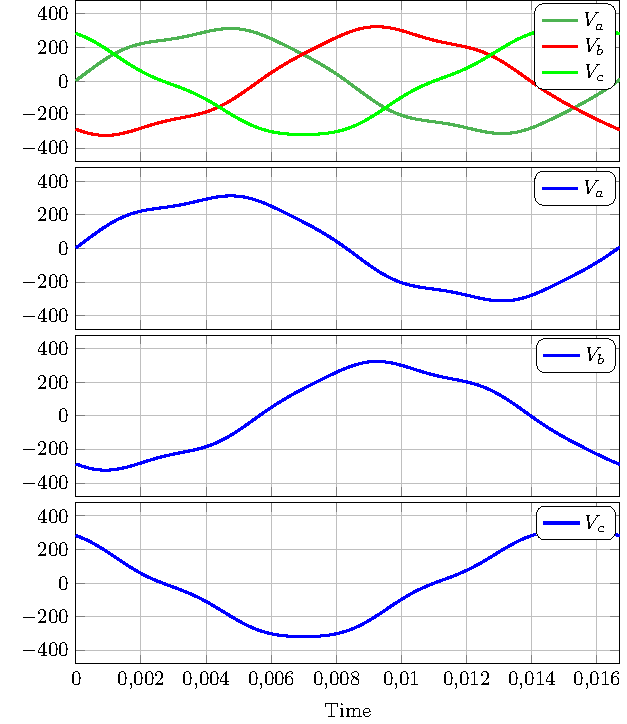
\includegraphics[width=\linewidth]{Capitulos/00/Figs/ex01}	
	\label{fig:ex01}
\end{figure}

Por exemplo, na \figref{fig:ex01}, tem-se...


\begin{figure}
	\centering
	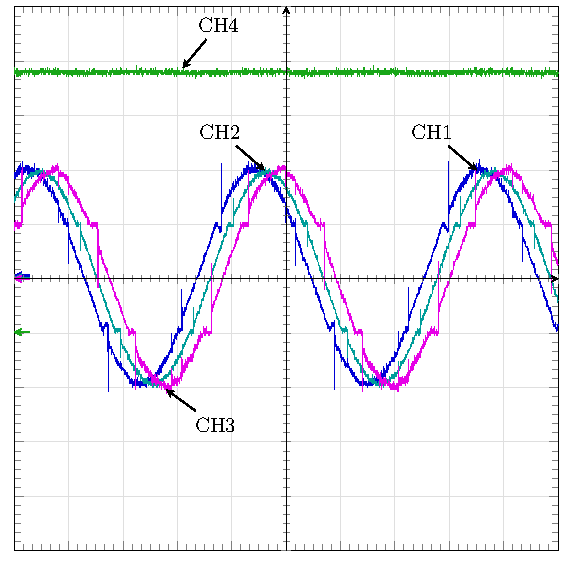
\includegraphics[width=0.9\linewidth]{Capitulos/00/Figs/tek0009}
	\caption{Exemplo de aquisição}
	\label{fig:tek0009}
\end{figure}

Este documento e seu código-fonte são exemplos de referência de uso da classe
\textsf{abntex2} e do pacote \textsf{abntex2cite}. O documento 
exemplifica a elaboração de trabalho acadêmico (tese, dissertação e outros do
gênero) produzido conforme a ABNT NBR 14724:2011 \emph{Informação e documentação
- Trabalhos acadêmicos - Apresentação}.

A expressão ``Modelo Canônico'' é utilizada para indicar que \abnTeX\ não é
modelo específico de nenhuma universidade ou instituição, mas que implementa tão
somente os requisitos das normas da ABNT. Uma lista completa das normas
observadas pelo \abnTeX\ é apresentada em \citeonline{abntex2classe}.

Sinta-se convidado a participar do projeto \abnTeX! Acesse o site do projeto em
\url{http://abntex2.googlecode.com/}. Também fique livre para conhecer,
estudar, alterar e redistribuir o trabalho do \abnTeX, desde que os arquivos
modificados tenham seus nomes alterados e que os créditos sejam dados aos
autores originais, nos termos da ``The \LaTeX\ Project Public
License''\footnote{\url{http://www.latex-project.org/lppl.txt}}.

Encorajamos que sejam realizadas customizações específicas deste exemplo para
universidades e outras instituições --- como capas, folha de aprovação, etc.
Porém, recomendamos que ao invés de se alterar diretamente os arquivos do
\abnTeX, distribua-se arquivos com as respectivas customizações.
Isso permite que futuras versões do \abnTeX~não se tornem automaticamente
incompatíveis com as customizações promovidas. Consulte
\citeonline{abntex2-wiki-como-customizar} par mais informações.

Este documento deve ser utilizado como complemento dos manuais do \abnTeX\ 
\cite{abntex2classe,abntex2cite,abntex2cite-alf} e da classe \textsf{memoir}
\cite{memoir}. 

Esperamos, sinceramente, que o \abnTeX\ aprimore a qualidade do trabalho que
você produzirá, de modo que o principal esforço seja concentrado no principal:
na contribuição científica.

Equipe \abnTeX 

Lauro César Araujo


